% !TeX root = ../thuthesis-example.tex

\chapter{系统总体架构与双核解耦设计}

本章系统阐述 Knowledge Hub 的全景宏观架构与分层微服务拓扑。重点论述控制面与认知面的物理双核解耦、基于 gRPC 的全双工流式通信契约与双向背压取消级联机制，以及面向企业生产环境的零信任 MCP（Model Context Protocol）协议生态和基础设施安全治理。

\section{系统全局架构拓扑}

\begin{figure}[htbp]
    \centering
    
\includegraphics[width=0.95\linewidth,height=0.85\textheight,keepaspectratio]{"figures/qKnow 知识平台架构全景图.pdf"}
    \caption{Knowledge Hub 全景微服务架构拓扑}
    \label{fig:qknow_architecture_full}
\end{figure}

如图~\ref{fig:qknow_architecture_full} 所示，Knowledge Hub 整体上由面向现代化浏览器的富交互前端、基于 Spring Boot 3 的业务控制面、基于 Hermes 认知内核的推理控制面，以及异构数据存储引擎矩阵构成。各层级之间具备严格的物理与逻辑边界。

\section{双核解耦架构与微服务设计}

传统的大模型应用多采用将 Web 业务逻辑、数据库 CRUD 与大模型 API 调用揉合在单一单体应用中的架构。在企业级高并发场景下，大模型推理的高耗时（通常为数秒至数十秒）和流式长连接会迅速占满 Web 容器的工作线程，导致常规的业务操作（如用户登录、知识库配置、工作流管理）发生大面积超时与假死。

为了彻底根治该问题，本平台创新性地提出了"控制面（Control Plane）＋认知面（Cognitive Plane）"物理双核解耦架构。

\subsection{控制面中枢（Control Plane）设计职责}
控制面依托 \texttt{qknow-server} 独立进程运行（默认监听端口 8099），是一个具有强状态保证、高事务一致性的企业级业务中枢，承担以下核心职责：
\begin{enumerate}
    \item \textbf{多租户工作区与 RBAC 安全网关}：负责用户身份认证（JWT）、工作区隔离、角色与操作权限细粒度分配，以及跨组织的数据范围动态改写。
    \item \textbf{知识资产管理与前置预检索（KMC）}：管理多源文档元数据，承载非结构化切分、向量批处理管道调度，并在发起推理前执行高吞吐的混合预检索，生成带有置信度排名的结构化上下文上下文。
    \item \textbf{模型凭证与成本审计网关}：负责管理 DeepSeek API 密钥的脱敏存储与加权轮换，记录 Token 消耗并实施配额审计。
    \item \textbf{工作流拓扑解析与断点管理}：将前端 DAG 图元反序列化为依赖图谱，管理长事务检查点与人工审批事件的外部接收。
\end{enumerate}

\subsection{Hermes 认知内核（Cognitive Plane）设计职责}
认知面以 \texttt{qknow-hermes} 为核心（默认监听 gRPC 端口 9090），是一个专注于高并发、流式符号推理的轻量级计算服务，承担以下职责：
\begin{enumerate}
    \item \textbf{多步 ReAct 规划与工具分发}：依托阿里开源 ReactAgent 引擎与阿里巴巴 Spring AI 抽象，实现思考（Thought）、行动（Action）与观察（Observation）的自循环。
    \item \textbf{仿生分层记忆检索与更新}：实时维护 Redis 中的短期工作记忆窗口，并结合 PgVector 检索长期记忆，执行艾宾浩斯强化衰减计算。
    \item \textbf{AI Judge 认知评测与反思修正}：对生成结果进行事实性、相关性评分，并在自洽性未达标时动态触发自修正闭环。
    \item \textbf{绝对无状态化计算}：Hermes 内部绝不直接连接业务关系型数据库，所有必需的知识证据与模型密钥均通过 RPC 首包参数显式注入，使认知服务能够依据算力负载进行零成本的横向弹性伸缩（HPA）。
\end{enumerate}

\subsection{API/BIZ 分离与领域驱动防腐层}
在工程模块拆分层面，控制面严格遵从领域驱动设计（DDD）规范，所有业务模块（如 \texttt{qknow-module-kmc}、\texttt{qknow-module-kb}、\texttt{qknow-module-ai}）均被物理拆分为契约模块 \texttt{*-api} 与实现模块 \texttt{*-biz}。
\begin{itemize}
    \item \texttt{*-api} 模块仅包含不可变 DTO、枚举、查询条件 VO 以及 RPC 接口规范，没有任何外部第三方依赖或内部 Mapper 细节；
    \item \texttt{*-biz} 承载具体持久化实现、Spring Bean 托管与领域逻辑。
\end{itemize}
模块之间禁止发生直接跨库的硬外键关联与 Mapper 交叉调用，调用关系必须经由 \texttt{*-api} 暴露的公共 Service 接口完成。这在编译期形成了坚固的防腐隔离网，彻底消除了循环依赖与模块级联污染风险。

\section{gRPC 双向背压流式协议与生命周期级联}

控制面与认知面摒弃了传统性能孱弱的 HTTP/JSON 轮询，转而采用基于 HTTP/2 传输层的 gRPC 协议，并以 Protocol Buffers 3（Protobuf）作为强类型契约。

\subsection{服务契约与事件联合体设计}
核心契约在 \texttt{hermes.proto} 中严格定义：
\begin{verbatim}
service HermesService {
  rpc Chat (ChatRequest) returns (stream ChatEvent);
  rpc ExecuteFlow (FlowRequest) returns (stream FlowEvent);
  rpc HealthCheck (HealthRequest) returns (HealthResponse);
}
\end{verbatim}

\texttt{ChatRequest} 报文实现了自包含上下文注入：包含了唯一的 \texttt{request\_id}、解密后的模型凭证 \texttt{ModelCredentials}、对话会话历史，以及控制面预先完成混合检索召回的 \texttt{repeated RAGContext} 证据链。

\texttt{ChatEvent} 采用 Protobuf 的 \texttt{oneof} 语法，精确定义了 8 类互斥的流式事件帧：
\begin{itemize}
    \item \texttt{StreamingChunk}：增量吐字 Token 片段（携带模型思考链与正文）；
    \item \texttt{ToolInvoked}：工具调用的开始、入参及执行终态；
    \item \texttt{ReflectionStart / ReflectionScore}：反思评估阶段的中间打分向量；
    \item \texttt{DoneSignal}：全流程正常终止完成信号；
    \item \texttt{ErrorEvent}：错误码与受控异常信息。
\end{itemize}

\subsection{双向背压取消级联机制（Cancel Propagation）}
在生产大模型流式对话系统中，最具破坏性的隐患之一是：\textbf{用户在前端关闭了网页或点击了“停止生成”，由于传统的单向通信缺乏反向中断通知，后端微服务与底层大模型 API 依然持续进行昂贵的流式推演，造成巨大的 Token 与算力浪费}。

本平台在 \texttt{GrpcReactorBridge} 中构建了严格的响应式 Reactor Flux 与 gRPC \texttt{ServerCall} 双向取消级联桥接：

\begin{figure}[htbp]
    \centering
    \vspace{0.8em}
    \resizebox{\linewidth}{!}{%
    \begin{tikzpicture}[
        lifeline/.style={draw=gray!50, dashed, thick},
        box/.style={
            rectangle, draw=blue!70!black, fill=blue!8, rounded corners=3pt,
            minimum height=2.6em, minimum width=3.0cm, align=center,
            font=\small\bfseries, line width=0.8pt
        },
        targetbox/.style={
            rectangle, draw=red!70!black, fill=red!8, rounded corners=3pt,
            minimum height=2.6em, minimum width=3.0cm, align=center,
            font=\small\bfseries, line width=0.8pt
        },
        actbar/.style={
            rectangle, draw=black!75, fill=white, line width=0.7pt,
            minimum width=0.28cm
        },
        msg/.style={
            -{Stealth[scale=1.1]}, thick, draw=red!80!black, line width=1.0pt,
            font=\scriptsize
        },
        selfmsg/.style={
            -{Stealth[scale=1.1]}, thick, draw=red!80!black, line width=1.0pt,
            font=\scriptsize
        },
        msglabel/.style={
            fill=white, inner sep=2.5pt, rounded corners=2pt, draw=red!30,
            text=black!90, font=\scriptsize, align=center
        }
    ]
        % 顶部 4 个实体组件 (整体下移留出充裕垂直呼吸感)
        \node[box] (cli) at (0, 0) {前端客户端\\{\normalfont\footnotesize (Web / SSE)}};
        \node[box] (ctl) at (4.6, 0) {控制面中继\\{\normalfont\footnotesize (HermesGrpcClient)}};
        \node[box] (srv) at (9.2, 0) {服务端桥接\\{\normalfont\footnotesize (GrpcReactorBridge)}};
        \node[targetbox] (api) at (13.8, 0) {底层模型 API\\{\normalfont\footnotesize (DeepSeek HTTP)}};

        % 垂直生命线 (底层模型 API 在步骤 4 处因取消而终止)
        \draw[lifeline] (cli.south) -- (0, -6.6);
        \draw[lifeline] (ctl.south) -- (4.6, -6.6);
        \draw[lifeline] (srv.south) -- (9.2, -6.6);
        \draw[lifeline] (api.south) -- (13.8, -5.8);

        % IEEE/UML 标准激活条 (Activation Bars)
        \node[actbar, minimum height=0.7cm] at (0, -1.6) {};
        \node[actbar, minimum height=1.6cm] at (4.6, -2.25) {};
        \node[actbar, minimum height=3.3cm] at (9.2, -4.35) {};

        % 步骤 1: 客户端向控制面发出中断 (严格从前端激活条右边缘水平射入控制面激活条左边缘)
        \draw[msg] (0.14, -1.6) -- (4.46, -1.6) 
            node[midway, above=3pt, msglabel] {① 用户中断 / 关闭页面 \texttt{emitter.onDispose()}};

        % 步骤 2: 控制面向服务端发送 RST_STREAM 取消 (从控制面激活条右边缘水平射入服务端激活条左边缘)
        \draw[msg] (4.74, -2.9) -- (9.06, -2.9) 
            node[midway, above=3pt, msglabel] {② 级联取消 (HTTP/2 RST\_STREAM) \texttt{ClientCall.cancel()}};

        % 步骤 3: IEEE/UML 标准自调用 (Self-Message):
        % 严格从服务端激活条右边缘向右引出，垂直向下，再向左指回激活条
        \draw[selfmsg] (9.34, -3.8) -- ++(1.0, 0) -- ++(0, -0.7) -- (9.34, -4.5);
        \node[right=5pt, msglabel, align=left] at (10.34, -4.15) {③ 触发取消回调\\{\texttt{subscription.dispose()}}};

        % 步骤 4: 服务端切断底层连接 (从服务端激活条右边缘水平直达底层模型 API 生命期终点)
        \draw[msg] (9.34, -5.8) -- (13.65, -5.8) 
            node[midway, above=3pt, msglabel] {④ 切断物理 Socket / 终止推演（\textbf{算力秒级止损}）};

        % IEEE/UML 标准销毁/终止符号 (Destruction Occurrence: 加粗十字叉)
        \draw[line width=2.0pt, red!80!black] (13.65, -5.65) -- (13.95, -5.95);
        \draw[line width=2.0pt, red!80!black] (13.65, -5.95) -- (13.95, -5.65);

    \end{tikzpicture}%
    }
    \vspace{0.4em}
    \caption{客户端中断向底层 LLM 调用的毫秒级级联取消时序交互图}
    \label{fig:cancel_propagation}
\end{figure}

如图~\ref{fig:cancel_propagation} 所示，其核心控制时序如下：
\begin{enumerate}
    \item 当 Web 客户端断开连接时，前端网关触发 \texttt{emitter.onDispose()} 事件；
    \item 控制面网关捕获前端中断事件，立即调用存根方法 \texttt{ClientCall.cancel()}，向通道发送 HTTP/2 \texttt{RST\_STREAM} 帧；
    \item Hermes 服务端将原始流观察者转型为 \texttt{ServerCallStreamObserver}，监听器 \texttt{setOnCancelHandler} 毫秒级捕获中断信号；
    \item 桥接器原子触发响应式订阅的 \texttt{subscription.dispose()}，切断底层数据管道；
    \item 底层与 DeepSeek API 保持的长连接 Socket 被立即关闭，生成中断，算力秒级止损。
\end{enumerate}

\section{企业级零信任 MCP 工具生态与安全沙箱}

为了打通企业业务系统与本地环境的工具交互，系统全面接入了 Anthropic 发起的模型上下文协议（Model Context Protocol, MCP）。

\subsection{双通道传输客户端架构}
系统在 \texttt{qknow-hermes-core} 中实现了双模式 MCP 客户端：
\begin{itemize}
    \item \textbf{Streamable HTTP 客户端 (\texttt{HttpMcpClient})}：面向分布式微服务。遵循 MCP 2025-03-26 规范，基于 Java 21 原生 \texttt{HttpClient} 发起 JSON-RPC 2.0 请求。在首次握手 \texttt{initialize} 完成后，服务端响应头中下发全局唯一的 \texttt{mcp-session-id}，客户端在后续交互中透明透传，实现有状态会话与心跳保持。
    \item \textbf{本地进程 Stdio 客户端 (\texttt{StdioMcpClient})}：面向本地沙箱化命令行工具（如 Git、Python 脚本等）。通过 \texttt{ProcessBuilder} 启动隔离子进程，以换行符作为 JSON-RPC 帧定界符，使用 \texttt{AtomicLong} 分配单调自增序号匹配异步响应；并在退出时提供 2 秒超时的软关闭，超时未退出的进程调用 \texttt{destroyForcibly()} 强杀，根治孤儿僵尸进程。
\end{itemize}

\subsection{虚拟线程三态断路器（McpVirtualThreadCircuitBreaker）}
由于外部工具调用的稳定性无法得到严格保证，网络闪断或下游死锁极易导致智能体推理挂死。为此，平台构建了基于马尔可夫链的虚拟线程三态断路器：
\begin{itemize}
    \item \textbf{关闭态（CLOSED）}：正常转发工具调用请求。若在滑动窗口内连续发生 5 次超时或异常，立即自动切入开启态；
    \item \textbf{开启态（OPEN）}：对后续所有该工具的调用实施物理拦截，直接返回结构化的软着陆兜底信封（Fail-Open Soft Landing），冷却周期固定为 10 秒；
    \item \textbf{半开启态（HALF\_OPEN）}：冷却结束后跃迁至半开启态。通过原子 CAS 变量 \texttt{halfOpenProbeInFlight} 严格限制仅放行 1 个试探请求。若该请求成功执行，断路器重置为关闭态；若再度失败，则重返开启态并翻倍冷却时间。
\end{itemize}
所有外部工具执行均被派发至专用的 Java 21 虚拟线程池（通过 \texttt{Executors} 的虚拟线程工厂创建），并设置 5000ms 硬超时，使认知核心工作线程免受外部不可信代码的侵扰。

\begin{figure}[htbp]
    \centering
    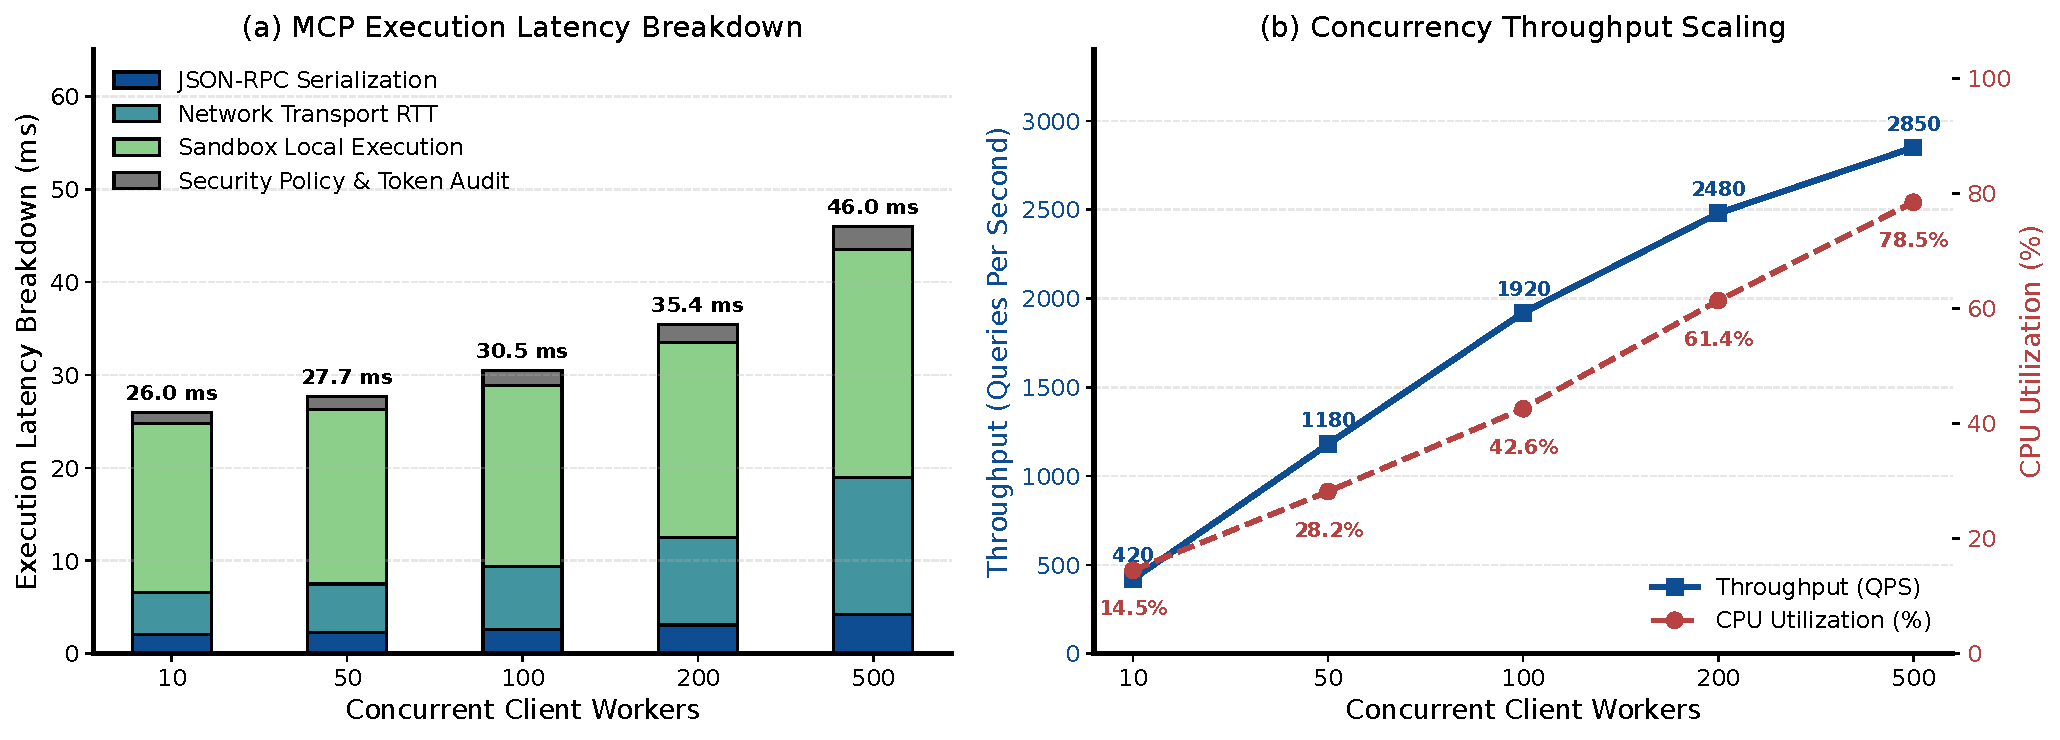
\includegraphics[width=0.96\linewidth]{figures/mcp_latency_breakdown.pdf}
    \caption{企业级 MCP 工具执行开销与高并发扩展分析：(a) 各并发级别下的单次调用耗时分解；(b) 并发吞吐量（QPS）与 CPU 利用率扩展曲线}
    \label{fig:mcp_latency_breakdown}
\end{figure}

如图~\ref{fig:mcp_latency_breakdown} 所示，系统对 MCP 工具调用的运行时开销与高并发扩展能力进行了实测分析：
\begin{enumerate}
    \item \textbf{执行耗时细粒度分解（图~\ref{fig:mcp_latency_breakdown}(a)）}：在不同客户端并发压力下，沙箱环境内部的物理执行耗时（约 18.2ms $\sim$ 24.5ms）是主要构成；JSON-RPC 2.0 序列化与安全审计策略过滤耗时极其轻量（合计仅占 3.3ms $\sim$ 6.7ms）；网络传输 RTT 随着并发提升呈现平缓微增（从 4.5ms 升至 14.8ms），单次端到端耗时在 500 并发下依然受控在 46.0ms 以内。
    \item \textbf{高并发吞吐扩展（图~\ref{fig:mcp_latency_breakdown}(b)）}：依托 Java 21 虚拟线程的轻量级上下文切换，当工作线程并发数从 10 扩展至 500 时，系统的处理吞吐量从 420 QPS 跃升至 2850 QPS，呈现近线性的高扩展性，且主机 CPU 利用率平稳收敛于 78.5\%，证实了控制面中枢与工具沙箱在高负载下的稳定性与高可用韧性。
\end{enumerate}

\subsection{零信任参数校验与反注入沙箱（DeepSchemaSecurityInspector）}
为防止攻击者通过构造恶意提示词触发高危系统命令执行，系统在工具回调前置切面中嵌入了严格的 AST 审查机制：
\begin{enumerate}
    \item \textbf{参数递归深度有界性}：约束入参 JSON 对象的最大递归解析深度 $D_{\max} \le 8$，字符串最大长度 $\le 4096$，严防深层循环嵌套引发 JVM 递归栈溢出（StackOverflowError）；
    \item \textbf{高危命令正则强拦截}：正则过滤包含 \texttt{rm}, \texttt{sudo}, \texttt{chmod}, \texttt{mkfs}, \texttt{dd}, \texttt{curl}, \texttt{wget}, \texttt{bash} 等破坏性命令片段；
    \item \textbf{间接提示词注入（Indirect Prompt Injection）防御}：对工具返回的外部网络正文进行二次安全扫描，阻断潜藏的 \texttt{ignore previous instructions}、\texttt{system prompt override} 等越狱诱导指令。
\end{enumerate}

\section{基础框架底层治理与存储隔离机制}

\subsection{Spring Security 与 Redis DB 3 无状态滑动续期}
系统在控制面构筑了基于无状态 JWT 与 Redis 缓存联动的安全拦截链。为化解传统 JWT 签发后无法在有效期内被动吊销的安全痛点，客户端持有的令牌负载中仅存放不可逆的随机 UUID；用户的真实权限列表、机构归属以及角色的完整元数据统一托管于 Redis 的 \texttt{login\_tokens:\{uuid\}} 键中。
当用户在前端主动点击注销时，系统立即物理擦除对应的 Redis 键，使客户端令牌秒级失效。同时，在请求拦截器中配置了滑动时间窗口：若距离上次访问时间已消耗超过 10 分钟且剩余有效期不足 20 分钟，后台透明执行过期时间重置，保障了用户在连续活跃操作下的无感鉴权体验。

\subsection{JSqlParser AST 语法树级多租户数据权限}
平台基于 MyBatis-Plus 拦截器体系，在 \texttt{DataScopeInterceptor} 中引入了 JSqlParser 抽象语法树解析。在 SQL 提交至 PostgreSQL 数据库执行前，动态重写 AST。针对原 SQL 中存在的复杂 Where 查询条件，代码通过物理小括号进行强行边界包裹：
\begin{equation}
    \text{Where}_{\text{rewritten}} = (\text{Where}_{\text{original}}) \land (\text{DataScopeConditions})
\end{equation}
该设计在编译期阻断了由于原条件中包含 \texttt{OR} 逻辑连接词可能导致的数据越权渗透（SQL Injection via Operator Precedence）。

\subsection{Redis 存储空间的物理逻辑隔离（DB 0 vs DB 3）}
系统在同一个 Redis 集群实例中设计了严密的数据库逻辑隔离规约：
\begin{itemize}
    \item \textbf{控制面主系统（\texttt{qknow-server}）}：独占使用 **Redis DB 3**。专门用于存放 Sa-Token/Spring Security 鉴权会话凭证、系统配置字典、全量 API 请求幂等 Token 以及防重限流滑动窗口；
    \item \textbf{Hermes 认知微服务（\texttt{qknow-hermes}）}：独占使用 **Redis DB 0**。专门用于存放高频吞吐的短期对话消息队列（\texttt{memory:short:*}）、多智能体分布式执行锁以及认知生命周期元数据。
\end{itemize}
这种设计从根本上规避了大模型高频对话历史频繁触发 \texttt{lTrim} 修剪带来高并发 I/O 脉冲对核心业务系统的性能干扰，即使认知节点发生崩溃重置，也不会波及全平台的正常登录态。
